\documentclass[12pt]{amsart}

\addtolength{\hoffset}{-2.25cm}
\addtolength{\textwidth}{4.5cm}
\addtolength{\voffset}{-2.5cm}
\addtolength{\textheight}{5cm}
\setlength{\parskip}{0pt}
\setlength{\parindent}{15pt}

\usepackage{amsthm}
\usepackage{amsmath}
\usepackage{amssymb}
\usepackage[colorlinks = true, linkcolor = black, citecolor = black, final]{hyperref}

\usepackage{graphicx}
\graphicspath{ {./images/} }
\usepackage{multicol}
\usepackage{ marvosym }
\usepackage{wasysym}
\usepackage{tikz}
\usetikzlibrary{patterns}

\newcommand{\ds}{\displaystyle}
\DeclareMathOperator{\sech}{sech}

\setlength{\parindent}{0in}

\begin{document}

\thispagestyle{empty}

{\scshape Sotirios Moschos 9030} \hfill {\scshape \large Advanced Signal Processing} \hfill {\scshape Homework \#2}

\smallskip

\hrule

\bigskip

{\large\textbf{Plots}}

\bigskip

\textbf{Real discrete process X(k)}
\begin{figure}[h]
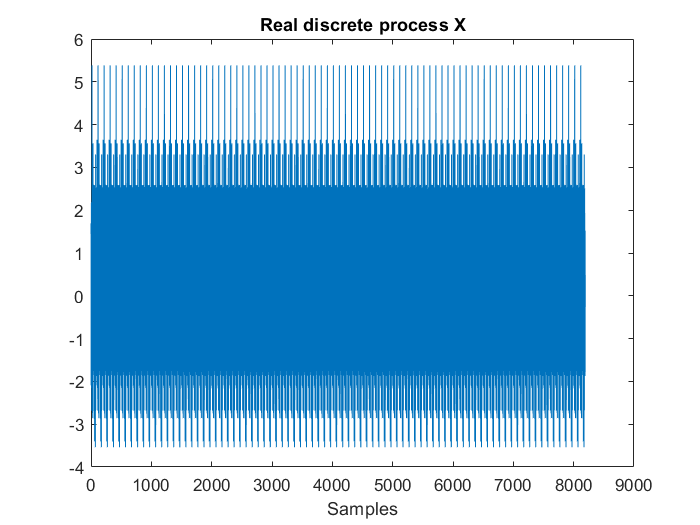
\includegraphics[width=8cm]{{Images/X(k).png}}
\end{figure}

In order to get the power spectrum we used the function SpectrumEstimator from the dsp toolbox.
We chose Welch's averaged modified periodograms method and Hann's window function.

\textbf{Power spectrum 1}
\begin{figure}[h]
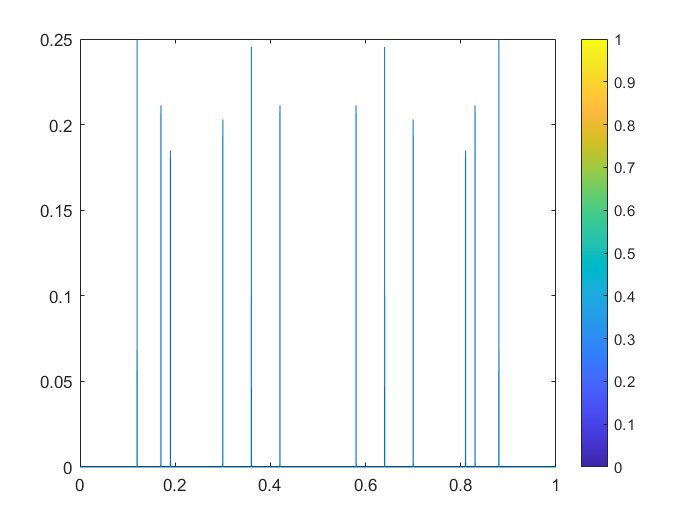
\includegraphics[width=8cm]{{Images/power spectrum 1.png}}
\end{figure}

In another approach, we calculated the the power spectrum via the FFT of the covariance of X(k). Hence, we got the following plot.

\textbf{Power spectrum 2}
\begin{figure}[h]
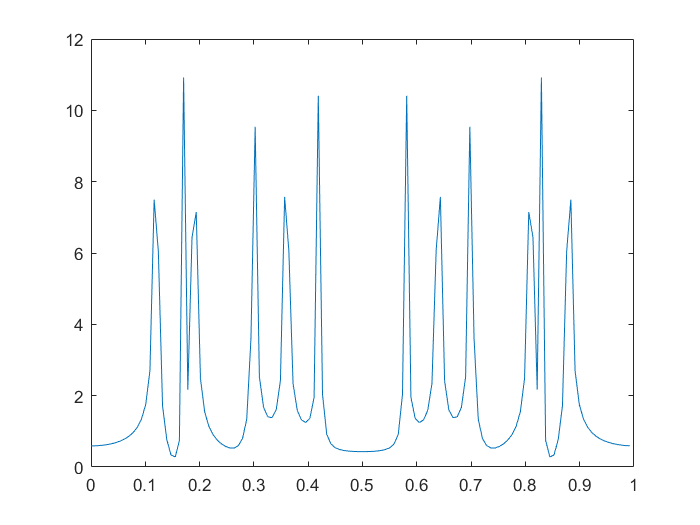
\includegraphics[width=8cm]{{Images/power spectrum 2.png}}
\end{figure}

\bigskip

{\large\textbf{Comparison of indirect bispectrum estimation methods}}

\bigskip

In order to get the following plots, we used the bispeci function from HOSA toolbox. For the first subtask we used the hexagonal window with unity values, as it's shape is similar to the rectangular window, so we can draw similar conjectures.\newline
For the second subtask we used the parzen window.\newline
Hence, we got the following plots: For the first plot we used the hexagonal window with unity values and for the second plot the parzen window.
\begin{figure}[h]
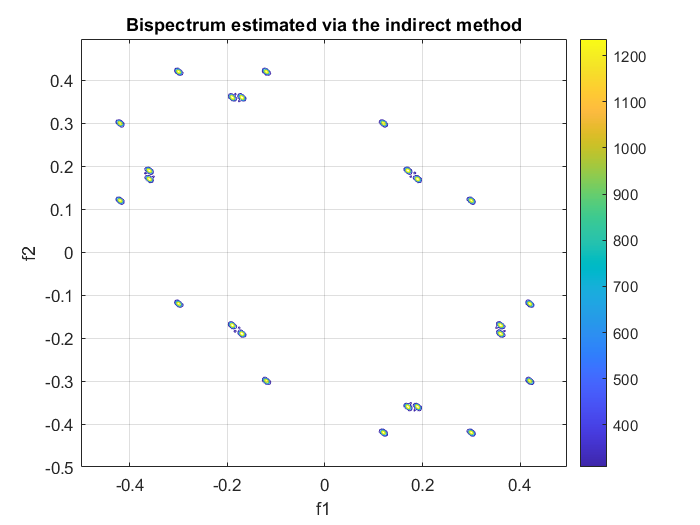
\includegraphics[width=8cm]{{Images/indirect-hexagonal.png}}
\end{figure}
\begin{figure}[h]
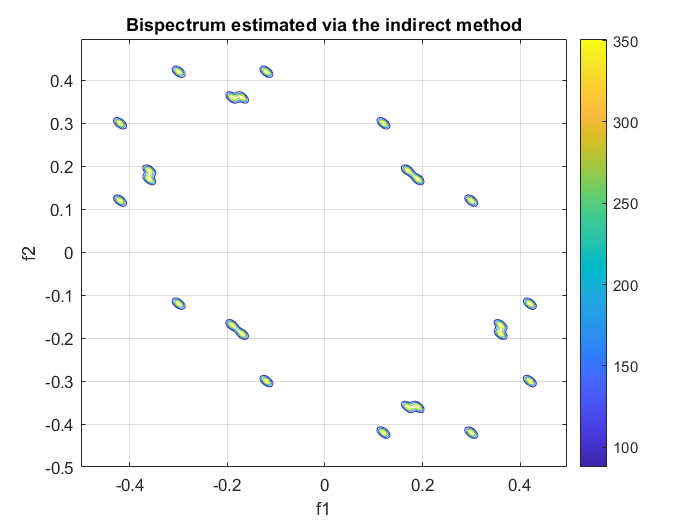
\includegraphics[width=8cm]{{Images/indirect-parzen.png}}
\end{figure}

The are particular advantages and disadvantages on the use of the proper 2D window. When a finite set of measured data is available, the problem of higher-order statistics estimation for a signal is a sensible one We should take into account the bias, the variance and other quality measures of the estimator, the bispectral resolution and finally, the leakage effect. As we can see from the plots the rectangular window has a higher frequency resolution than the Parzen window, the Parzen window offers the larger main lobe and the rectangular window has the larger spectral leakage effect. We obtained this information from the following paper:
(\textbf{Bispectral resolution and leakage effect of the indirect bispectrum estimate for different types of 2D window functions, 2008, Teofil-Cristian Oroian et all.}).

\bigskip
\newpage
{\large\textbf{Comparison of indirect and direct bispectrum estimation methods}}

\bigskip

In order to get the following plot, we used the bicpecd function from HOSA toolbox.
\begin{figure}[h]
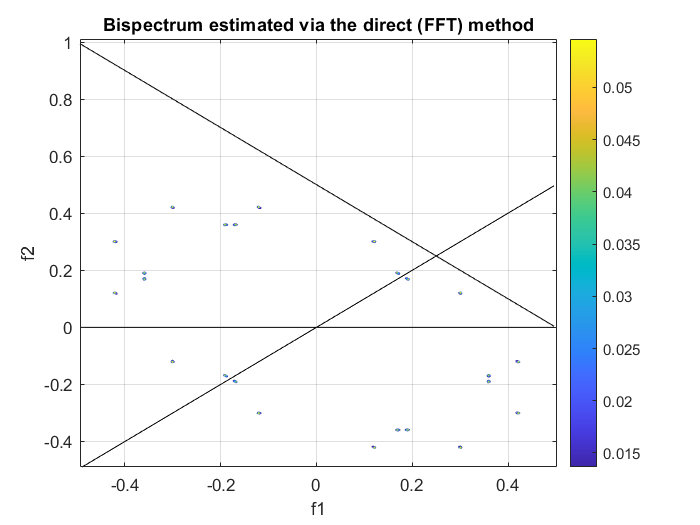
\includegraphics[width=8cm]{{Images/direct.png}}
\end{figure}\newline
We can state the the direct method has lower frequency resolution than the indirect method and the spectral leakage seems to be larger.

\bigskip

{\large\textbf{Frequency content of power spectrum vs bispectrum estimations}}

\bigskip

We can state that this homework assignment is a concrete application of signal processing namely, the quadratic phase coupling detection problem. In general, if we have a signal that is composed of three sinusoids with frequencies $\omega1,\omega2,\omega3$ and phases $\phi1,\phi2,\phi3$, the sinusoids 1 and 2 are said to be quadratically phase coupled (QPC) if and only if and \[\omega1+\omega2=\omega3\] \[\phi1+\phi2=\phi3\]
Analyzing the power spectrum plot, we can see that all 6 harmonics arise.
The bispectrum is a useful tool for QPC detection because only the phase couple components appear.  In our case, we can see that frequency resolutions appear on the frequency points: \[(\lambda1,\lambda2),(\lambda2,\lambda1)\,(\lambda3,-\lambda1),
(\lambda3,-\lambda2),(\lambda2,-\lambda3),(\lambda1,-\lambda3),\]
\[(-\lambda1,-\lambda2),(-\lambda2,-\lambda1),(-\lambda3,\lambda1)\,
(-\lambda3,\lambda2),(-\lambda1,\lambda3),(-\lambda2,\lambda3)\]
\[(\lambda4,\lambda5),(\lambda5,\lambda4)\,(\lambda6,-\lambda4),
(\lambda6,-\lambda5),(\lambda5,-\lambda6),(\lambda4,-\lambda6),\]
\[(-\lambda4,-\lambda5),(-\lambda4,-\lambda5),(-\lambda6,\lambda4)
,(-\lambda6,\lambda5),(-\lambda4,\lambda6),(-\lambda5,\lambda6)\]


\end{document}
